\documentclass[SE,authoryear,toc]{lsstdoc}
% GENERATED FILE -- edit this in the Makefile
\newcommand{\lsstDocType}{SITCOMTN}
\newcommand{\lsstDocNum}{166}
\newcommand{\vcsRevision}{1f7f2b0-dirty}
\newcommand{\vcsDate}{2025-09-18}


% Package imports go here.
\usepackage{amssymb,amsmath}

% Local commands go here.

%If you want glossaries
%\input{aglossary.tex}
%\makeglossaries

\title{Investigation of the Scratched Tape Scattered Light Artifact at Rubin Observatory}

% This can write metadata into the PDF.
% Update keywords and author information as necessary.
\hypersetup{
    pdftitle={Impact and Mitigation of the Scratched Tape Scattered Light Artifact},
    pdfauthor={Drlica-Wagner, A.},
    pdfkeywords={}
}

% Optional subtitle
% \setDocSubtitle{A subtitle}

\input{authors}

\setDocRef{SITCOMTN-166}
\setDocUpstreamLocation{\url{https://github.com/lsst-sitcom/sitcomtn-166}}

\date{\vcsDate}

% Optional: name of the document's curator
% \setDocCurator{The Curator of this Document}

\setDocAbstract{
 The ``scratched tape'' stray light feature is the most prominent and prevalent stray light artifact identified during the commissioning of the Vera C.\ Rubin Observatory. The scratched tape feature originates when light from large off-axis angles ($\sim$20\,deg) passes between the mid-level and center-section light baffles, reflects off of the primary mirror (M1), and illuminates the LSST Camera focal plane. This scenario represented an unobstructed light path to the sky during Rubin commissioning due to delays in the integration of the dome slit light--wind screen.  This document describes the identification, modeling, characterization, and proposed stop-gap mitigation strategy for the scratched tape stray light artifact.
 }

% Change history defined here.
% Order: oldest first.
% Fields: VERSION, DATE, DESCRIPTION, OWNER NAME.
% See LPM-51 for version number policy.
\setDocChangeRecord{%
  \addtohist{1}{2025-09-18}{Draft for release.}{Alex Drlica-Wagner}
  \addtohist{1}{2025-08-07}{Initial content.}{Alex Drlica-Wagner}
  \addtohist{1}{2025-07-09}{Initial template.}{Lee Kelvin}
}


\begin{document}

% Create the title page.
\maketitle
% Frequently for a technote we do not want a title page  uncomment this to remove the title page and changelog.
% use \mkshorttitle to remove the extra pages
%\mkshorttitle

% ADD CONTENT HERE
% You can also use the \input command to include several content files.

\section{Introduction}
\label{sec:introduction}

The unique, wide-field design of the Simonyi Survey Telescope at the Vera C.\ Rubin Observatory makes it particularly susceptible to stray and scattered light. Since one of the main science goals of Rubin is to investigate the low-surface-brightness universe \citep{2019ApJ...873..111I}, particular importance is placed on identifying, modeling, and mitigating stray-light artifacts. In particular, the delayed installation of the Rubin dome slit light--wind screen \citep[LWS;][]{Marchiori:2024} makes identifying and understanding stray light features particularly important during Rubin commissioning. A general overview of the identification and investigation of stray light features in Rubin commissioning can be found in \citet{SITCOMTN-160}. This note focuses specifically on efforts related to the ``scratched tape'' stray light feature, which is the most prominent and prevalent stray light artifact identified during Rubin commissioning and science validation.

The scratched tape artifact is a particular wide-area stray light feature that is present in at least 5\% of LSST Camera (LSSTCam) images taken during commissioning and early science validation (Figure~\ref{fig:tape}). It originates from an unobstructed light path to the sky that passes between the center-section and mid-level light baffles on the Telescope Mount Assembly (TMA) of the Simonyi Survey Telescope \citep{2022SPIE12182E..0WT}. The LWS is expected to block this path to the sky once it is installed and commissioned.  However, the partially completed state of the dome during commissioning and science validation allows astronomical sources located $\sim$20\,deg off-axis to illuminate the primary mirror (M1) and reflect directly into LSSTCam (i.e., bypassing M2 and M3). The result is a sharp, several-degree-long, rectilinear feature with surface brightness that has been measured at $\sim$20\% of the dark-sky background in some bands.
The scratched tape feature manifests in a variety of morphologies, brightnesses, and prominences (e.g., Figure~\ref{fig:tape}), and it may be related to several morphologically similar artifacts (e.g., the ``pillow'', ``muddy shoe'', etc.; \citealt{SITCOMTN-160}). In this document, we collectively use the term ``scratched tape'' to refer to all features that arise from the same off-axis stray light path.
Figure~\ref{fig:tape} show two morphologies of the scratched tape feature sourced by light from the bright star Alpha Centauri ($\alpha$Cen; $V \sim -0.1$\,mag) located $\sim$21\,deg off-axis.

\section{Identification of the Scratched Tape}
\label{sec:identification}

The scratched tape artifact was identified in early commissioning images from LSSTCam (the first documented instance was on 17 April 2025). The origin of this feature was originally unclear, though it was found to consistently impact specific fields (i.e., SV\_225\_-40). A visual inspection campaign was mounted to catalog and characterize the appearance of this and other stray-light features (see \citealt{SITCOMTN-160}). By correlating the appearance of the scratched tape with the locations of bright stars, it was determined that some of the brightest instances of the scratched tape appeared in observations taken when the bright star $\alpha$Cen ($V \sim -0.1$\,mag) was located $\sim$21\,deg off-axis. Based on this analysis, devoted observations were executed to reproduce the scratched-tape feature on 28 May 2025. While the ability to reproduce the feature strongly indicated that $\alpha$Cen was indeed the light source, the large off-axis light path responsible for this feature was still unclear.

\begin{figure*}[t!]
    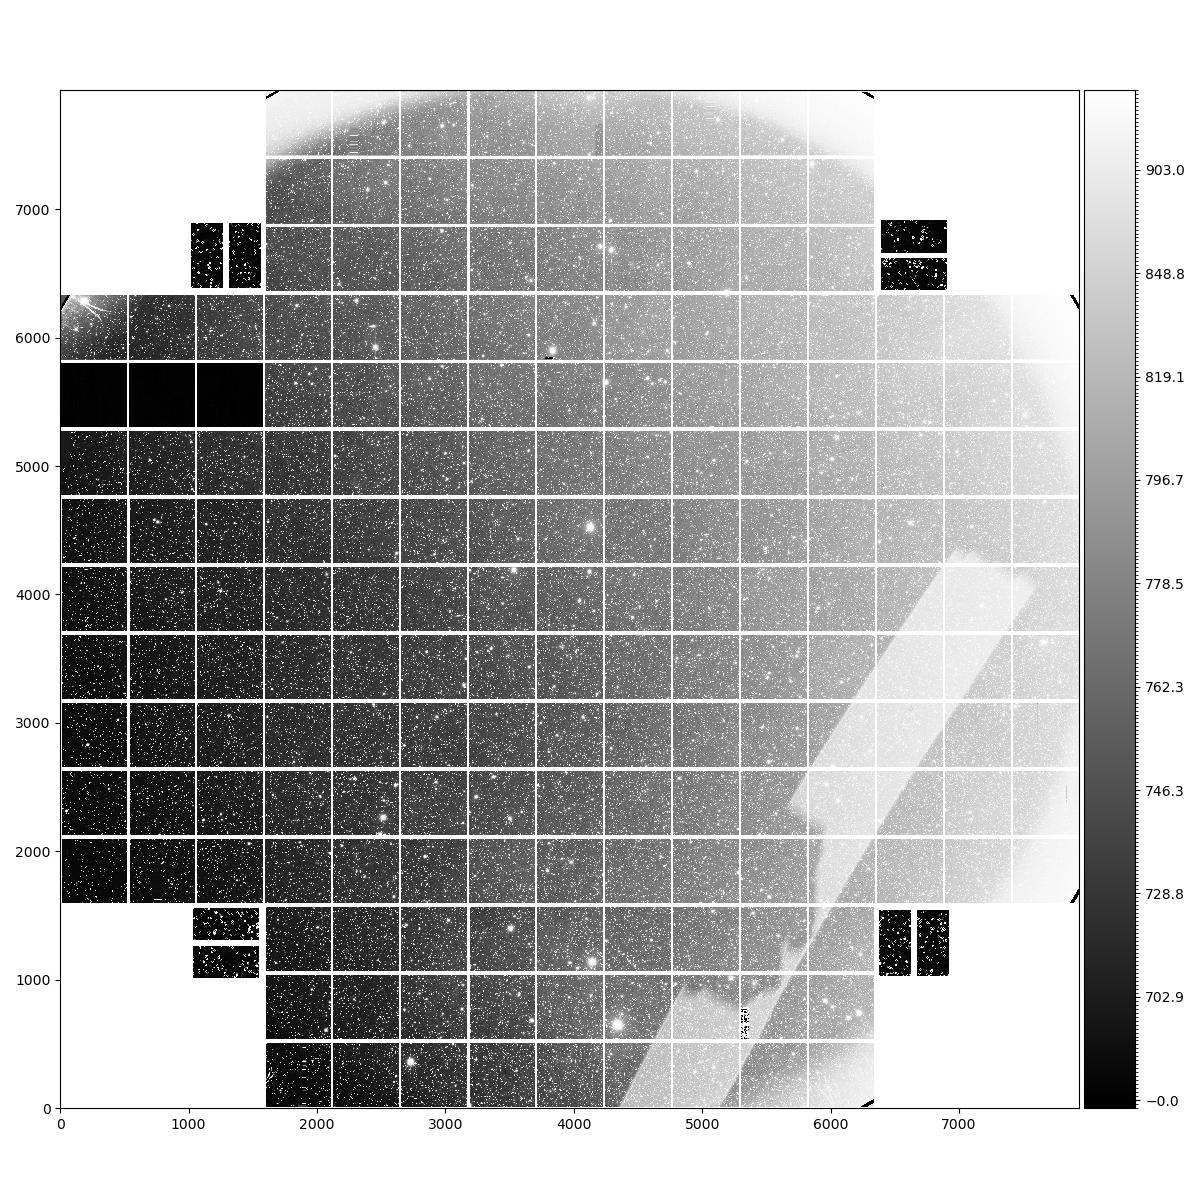
\includegraphics[width=0.49\textwidth]{figures/lsstcam_focal_plane_mosaic_2025-05-05_000421.jpg}
    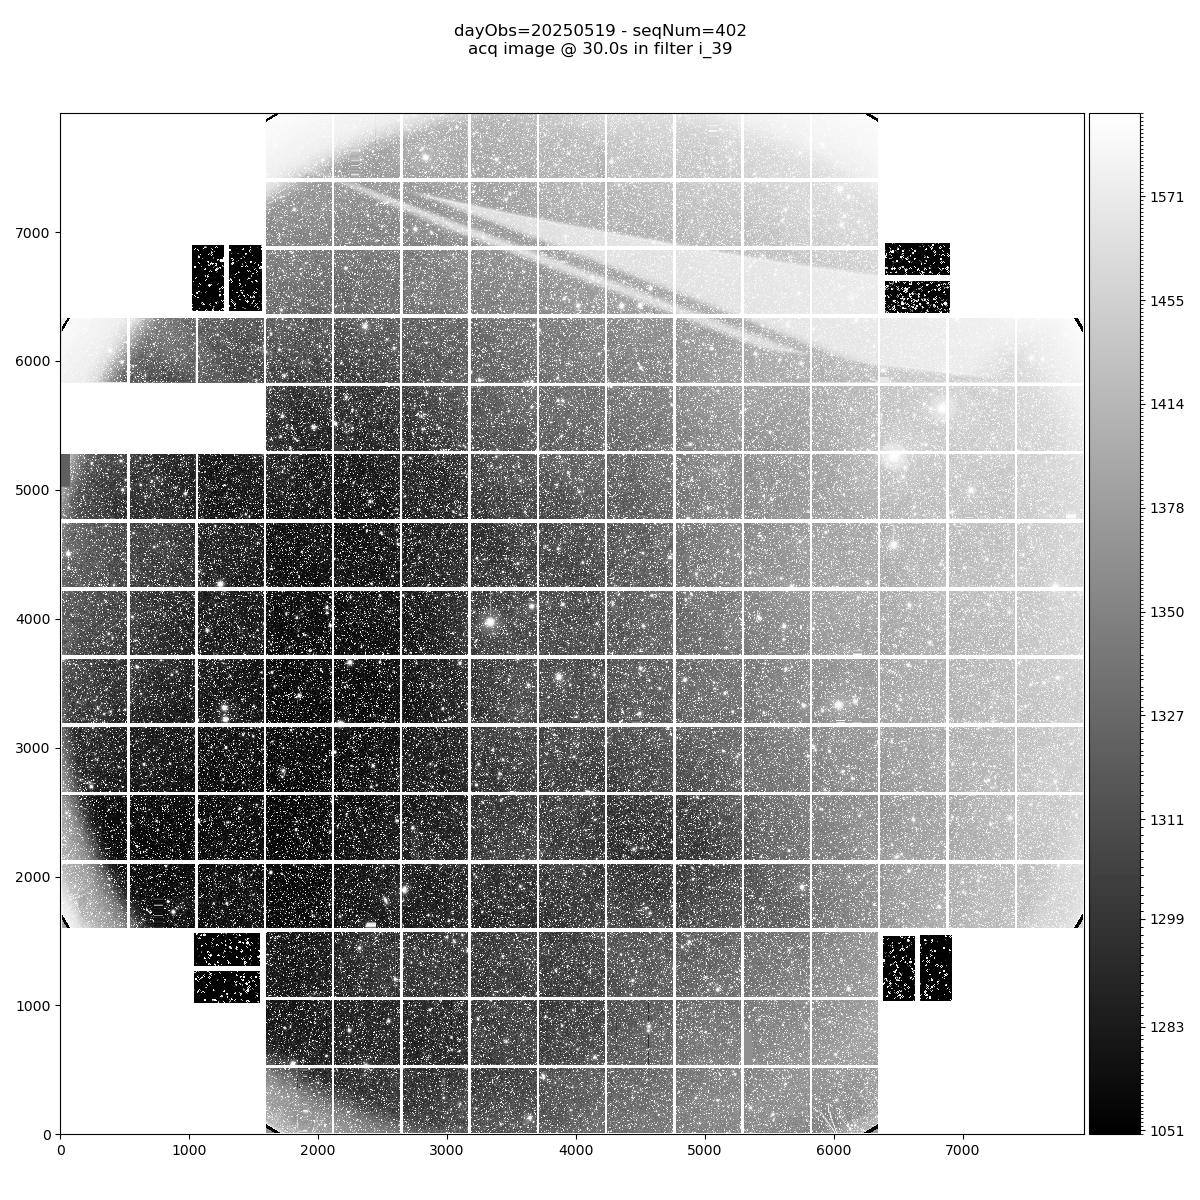
\includegraphics[width=0.49\textwidth, clip, trim={0.5cm 0 0 0}]{figures/lsstcam_focal_plane_mosaic_2025-05-19_000402.jpg}
    \caption{\label{fig:tape} Examples of stray light features associated with the ``scratched tape'' stray light path in LSSTCam images from Rubin commissioning. These examples originate from $\alpha$Cen ($V \sim -$0.1\,mag), which is located $\sim$21\,deg off-axis and illuminates M1 through a gap in the mid-level and center section light baffles. (Left) Prototypical ``scratched tape'' morphology (visit = 2025050500421). (Right) Prototypical ``sail'' morphology coming from a similar light path (visit = 2025051900402). The difference in morphology comes from physical obscuration by the TMA.}
\end{figure*}


\begin{figure*}[t!]
    \centering
    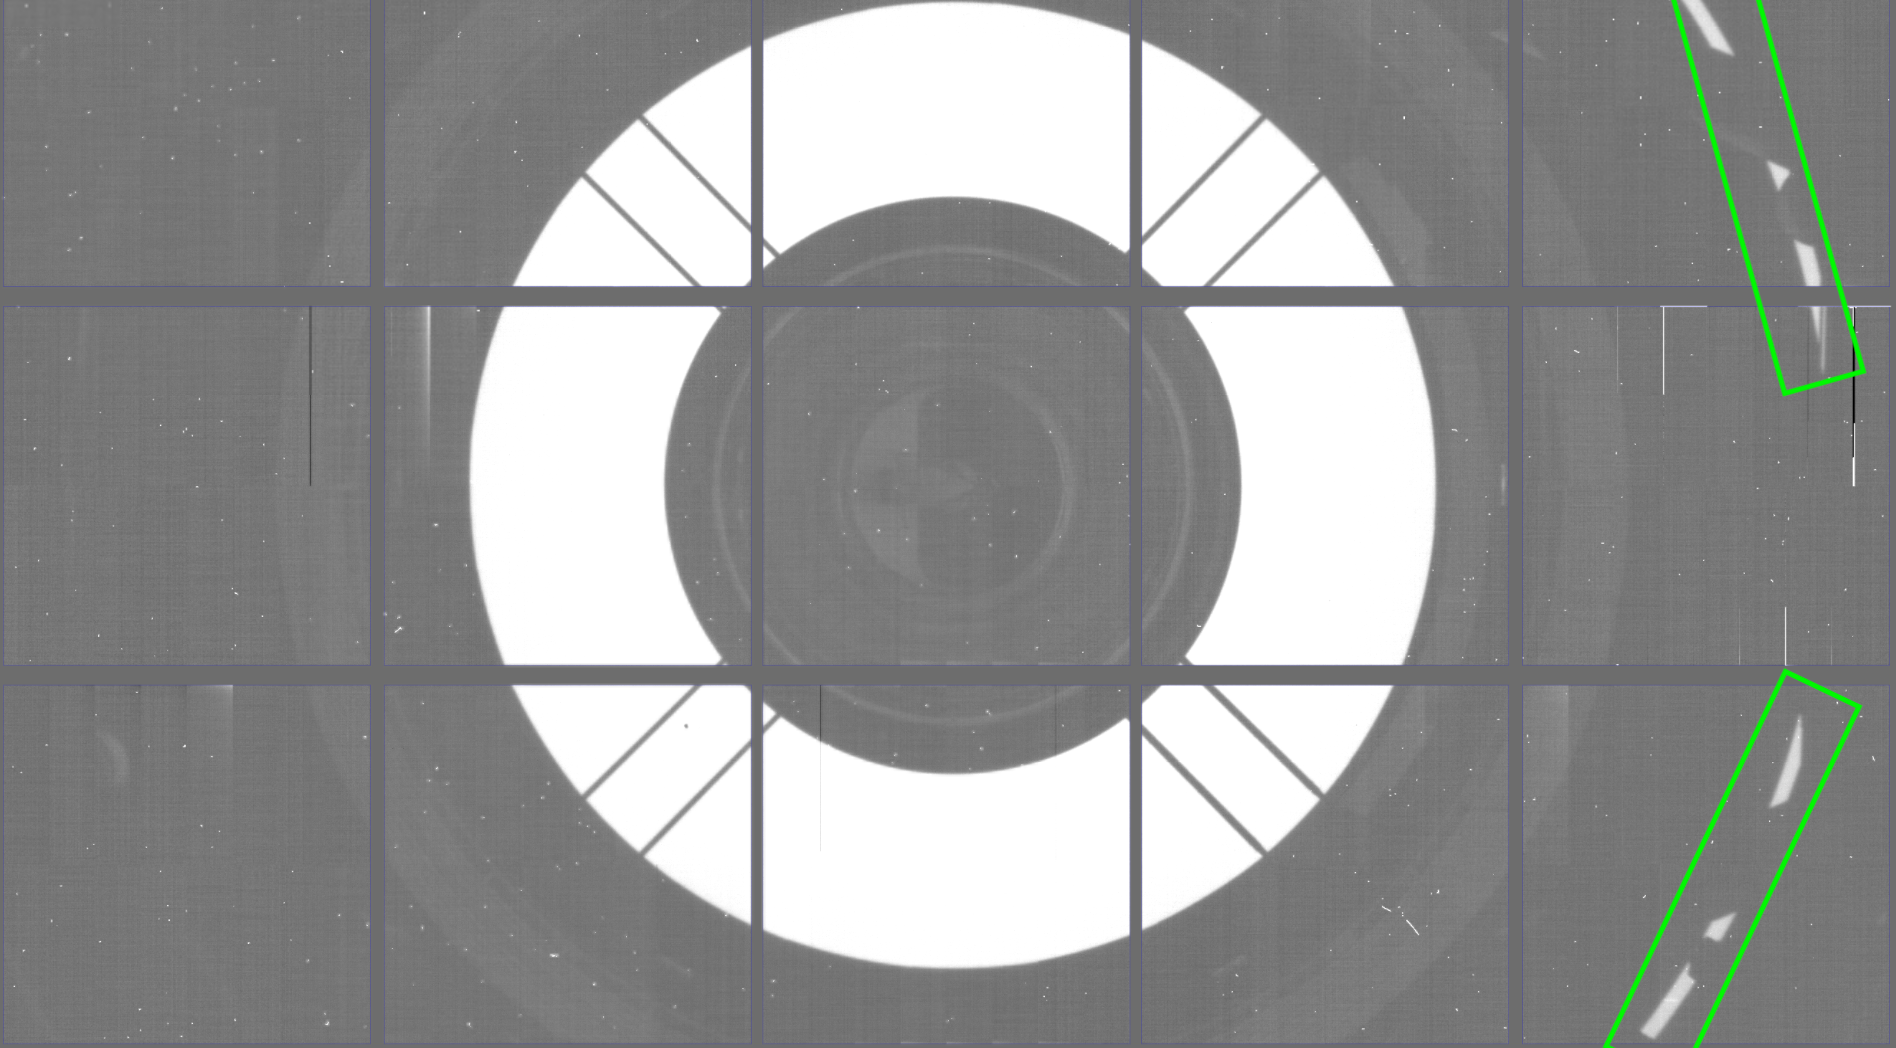
\includegraphics[width=0.75\textwidth]{figures/quicklook_2025070100103.png}\\[+0.5em]
    %https://usdf-rsp-dev.slac.stanford.edu/fov-quicklook/visits/raw:2025070100103?detectors=
    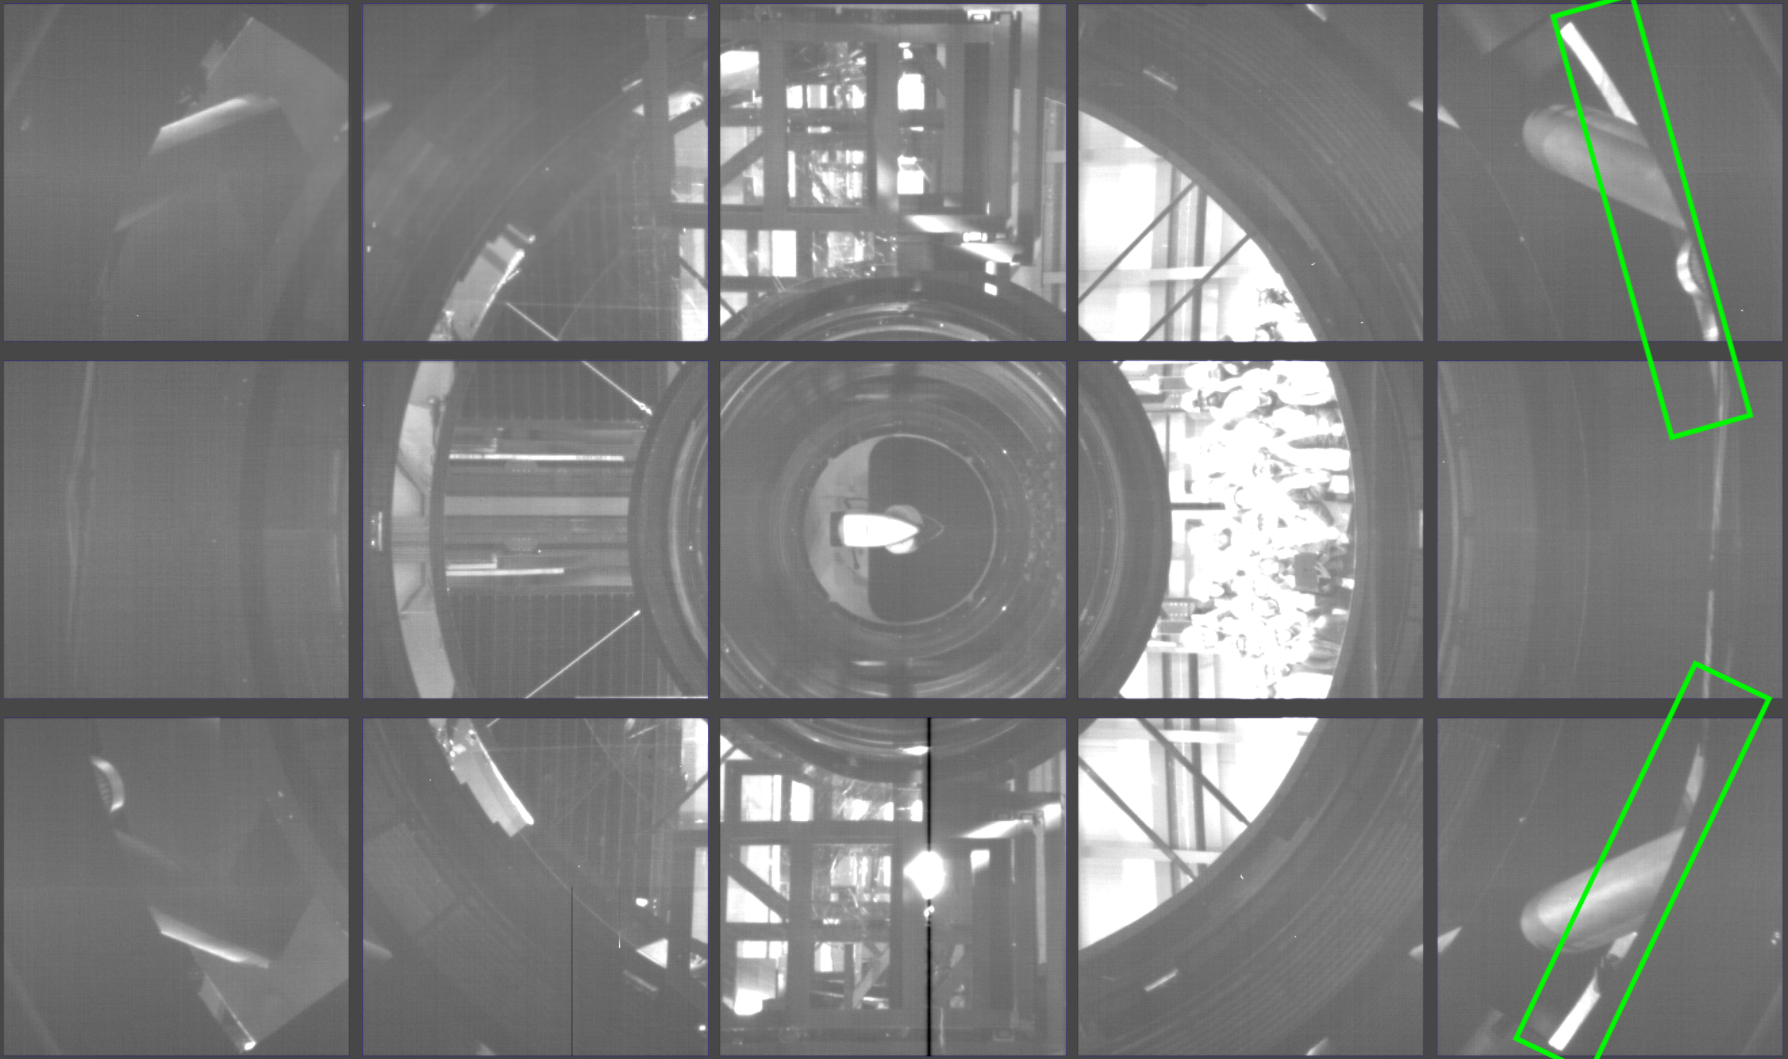
\includegraphics[width=0.75\textwidth]{figures/quicklook_2025070200040.png}  \caption{\label{fig:pinhole} Pinhole images showing the gap between the mid-level and center-section light baffles that is responsible for the scratched tape feature. (Top) Twilight flat (visit = 2025070100103) showing scratched-tape-like morphology coming from large incident angle. (Bottom) In-dome image at higher illumination level (visit = 20250702000040) showing the scratched tape path in the context of the TMA geometry.}
\end{figure*}

\section{Origin of the Scratched Tape}
\label{sec:cause}

After demonstrating the ability to reproduce the scratched tape feature on-sky, emphasis was placed on understanding the light path that allowed a bright star located $>$20\,deg off-axis to impact LSSTCam images. Investigation of images taken with the pinhole filter during twilight in early May 2025 proved extremely useful for this endeavor. The pinhole mask deployed for this test is inserted into the LSSTCam filter changer and produces an image of the telescope pupil, including the mechanical structures that surround the system clear aperture. We reconstructed a direct connection between the appearance of the scratched-tape features observed on-sky and the light patterns revealed by the pinhole images. Morphologically similar bright features were observed at large angles from the central pinhole in twilight images. Additional pinhole observations were executed in July 2025, including both on-sky twilight images and illuminated in-dome images. Investigation of these images identified the stray light path as a gap between the mid-level and center-section light baffle (Figure~\ref{fig:pinhole}). The existence of this gap was further experimentally verified by directed illumination with the collimated beam projector at large off-axis angles on 3 September 2025.


The scratched tape light path between the mid-level and center-section light baffles was reproduced with two independent ray-tracing models of the telescope and optical system (\texttt{batoid} and \texttt{Zemax}; Figure~\ref{fig:raytrace}). Note that while this gap extends more-or-less continuously around the entire mid-level ring of the TMA, the dome slit blocks light from the sky at large off-axis angles in azimuth. Modeling shows that the LWS is expected to block this path in altitude as well once it is installed and commissioned. Based on non-sequential \texttt{Zemax} modeling that includes a representative mechanical model of the TMA baffles and structure, the range of incident angles where this light path could illuminate the LSSTCam focal plane was determined to be 19.8\,deg $ \lesssim \theta \lesssim$ 26\,deg off-axis (Figure~\ref{fig:st_flux}). The \texttt{Zemax} modeling suggests that the angular range for bright scratched-tape features is concentrated between 20\,deg and 22\,deg, where the illumination can reach $\sim$10$^{-3}$ of the flux injected into the telescope pupil. Beyond 22\,deg, the illumination comes from secondary bounces off of structures internal to the camera, and the relative flux deposited onto the LSSTCam focal plane falls to $\sim$10$^{-6}$.

\begin{figure*}[t]
    \centering
    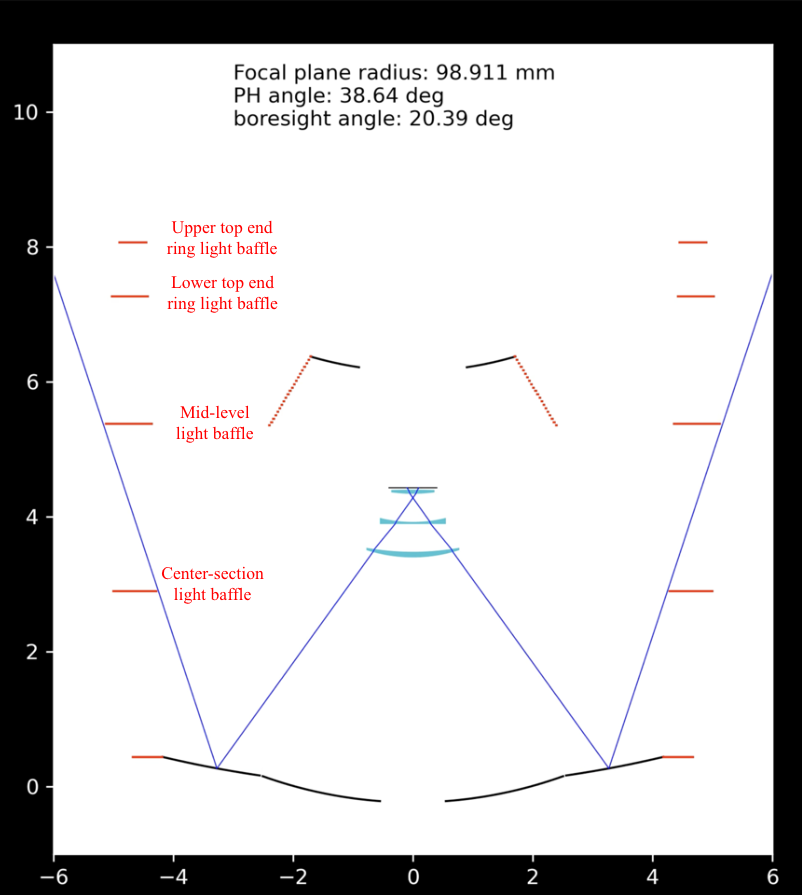
\includegraphics[width=0.43\textwidth]{figures/batoid_model.png}
    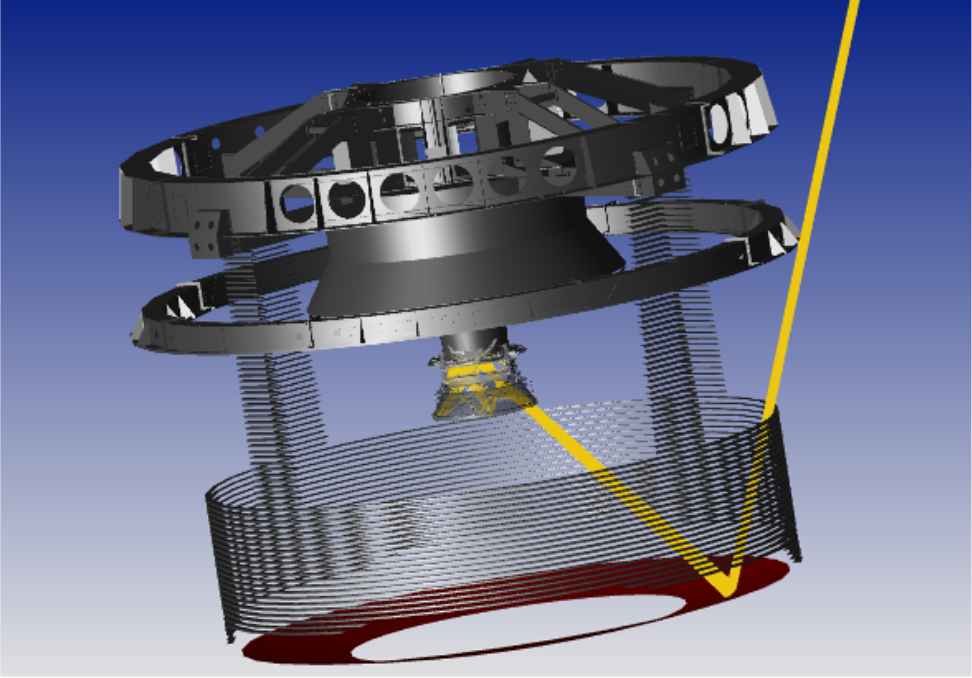
\includegraphics[width=0.56\textwidth, trim = {3.5cm 0cm 3cm 0cm}, clip]{figures/zemax_model.png}
    \caption{\label{fig:raytrace} Ray tracing models showing the scratched tape light path between the mid-level and center-section light baffles. (Left) The \texttt{batoid} model showing a ray passing through the scratched tape gap and into the center pinhole. The projected radius on the focal plane (98.911\,mm) corresponds to the position of the scratched tape seen in pinhole twilight flats. Baffles (red lines) are labeled following the nomenclature of LTS-213. (Right) The \texttt{Zemax} model showing the scratched tape light path with a more complete model of the TMA and LSSTCam. The \texttt{Zemax} modeling showed that it is possible for photons to reach the detectors for off-axis angles from 19.8 $< \theta <$ 26\,deg due to secondary bounces off of surfaces within the camera.}
\end{figure*}

\begin{figure}[!h]
    \centering
    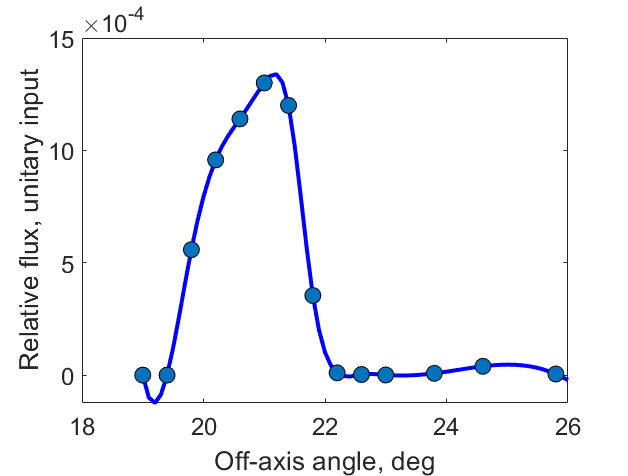
\includegraphics[width=0.7\textwidth]{figures/scratched_tape_flux.png}
    \caption{\label{fig:st_flux}Ray-tracing simulation with \texttt{Zemax} of the relative flux deposited onto the LSSTCam focal plane via the scratched tape light path for a unitary flux injected into the telescope pupil. Beyond 22\,deg the relative flux reaching the LSSTCam focal plane falls to $\sim$10$^{-6}$.
}
\end{figure}

Note that any light source placed within this angular range (and at appropriate altitude and azimuth to avoid other obstructions on the TMA) will illuminate the camera and is expected to produce scratched-tape-like features. However, only bright sources (e.g., bright stars, the Moon, the twilight sky, etc.) are sufficiently bright to be recognized by eye in the LSSTCam images. There are some indications that fields with many repeated observations taken with similar telescope altitude and azimuth (i.e., the Deep Drilling Fields) may have low-surface-brightness stray-light features that only become apparent after image coaddition.

\begin{figure*}[th]
    \centering
    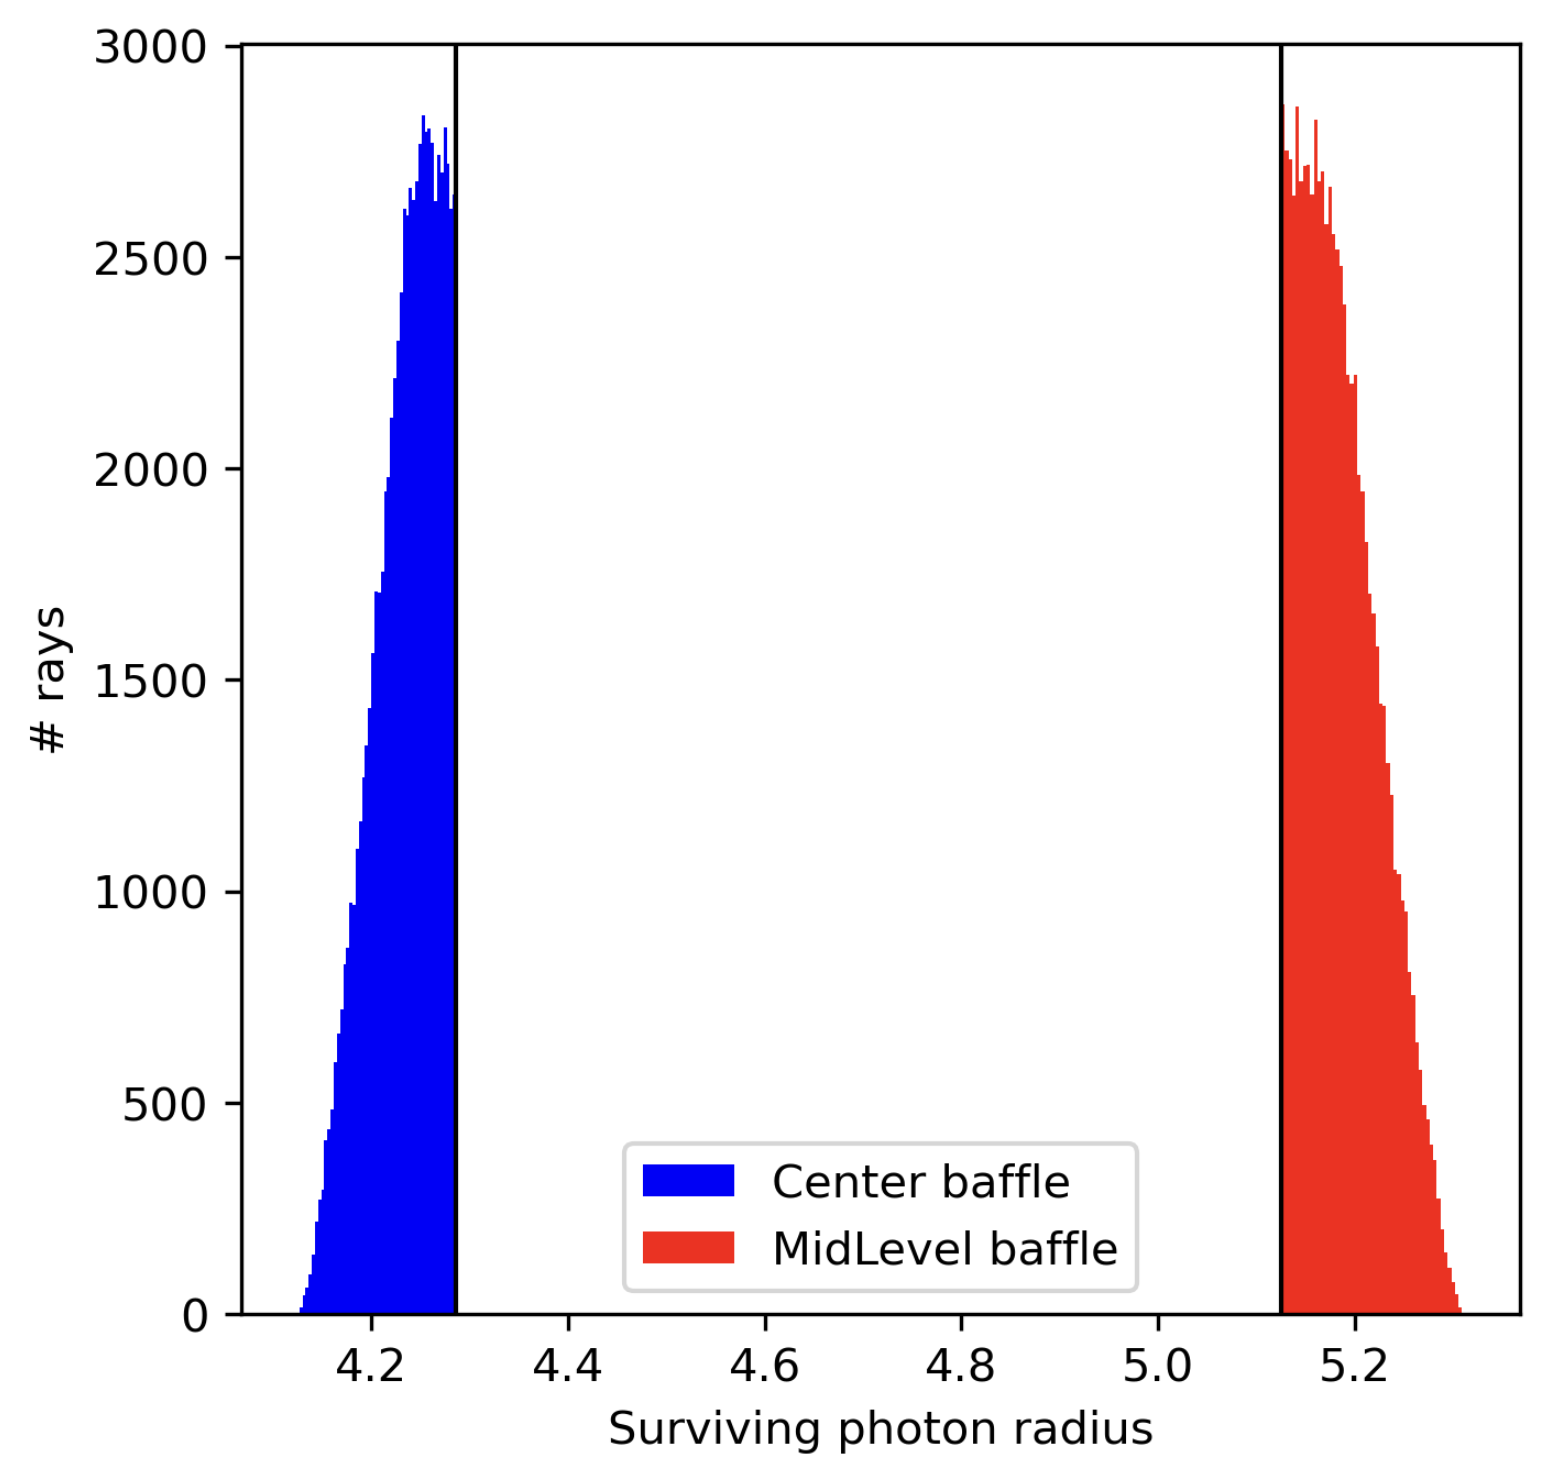
\includegraphics[width=0.5\textwidth]{figures/Baffle Gap Rays.png}
    \caption{Ray-tracing simulation run with \texttt{batoid} showing the distribution of $\sim 2\times 10^7$ photons fired in the direction of the scratched tape gap between the mid-level and center-section light baffle. The simulation tracks those rays that survive the trip through the baffles off of M1 into the LSSTCam and reached the detectors. This figure shows the radial distribution of the surviving rays at the heights of the mid-level Baffle (red) and the center-section baffle (blue). To block all of these photons, the mid-level baffle would need to be extended outward by 185\,mmm. However, note that these simulations use design dimensions of the TEA (LTS-213) and do not account for 10\,mm uncertainty on the TEA components.
}
\end{figure*}

\section{Characterizing the Scratched Tape Artifact}
\label{sec:brightness}

Extensive visual inspection has led to a large database of images affected by scratched tape and other related stray light artifacts (see SITCOMTN-160 for more details). During the period from 2025-04-17 to 2025-07-03, there were 1,093 documented examples of scratched tape out of 22,308 exposures ($\sim$4.9\%). However, much of the observing during commissioning was highly biased toward a small number of fields, and it can be argued that a more useful metric is the number of \emph{fields} in which the scratched tape occurs. Grouping together visits with boresight pointing (RA, Dec) within 0.2\,deg of each other, it was found that there are 2,998 unique sky configurations, of which 188 show the scratched-tape artifact ($\sim$6.3\%). Due to our evolving knowledge of the scratched tape morphology and origin, early visual classifications split the scratched tape into several morphologically distinct features that resulted from the same light path. Since the above analysis was performed only for features that were labeled ``scratched tape'', it likely underestimates the true incidence of related features. Due to a variety of factors (i.e., the brightness and location of the aggressor light source), the scratched tape can take on a variety of sizes, morphologies, and focal plane coverage fractions.  Furthermore, as flat fielding improved over the course of commissioning, it became possible to identify fainter scratched tape artifacts. Due to these complexities, the above analysis makes no attempt to capture the relative impact of each scratched tape occurrence.

While there is extensive knowledge of the occurrence rate of the scratched tape from systematic visual inspection of LSSTCam images, analyses of the flux and surface brightness of this feature are more limited due to the human effort involved. Early estimates came from aperture photometry of the scratched tape feature associated with $\alpha$Cen (visit = 2025051900386) found a total flux of 1.4 $\times$ 10$^{10}$ counts in $r$-band. This is approximately 0.2\% (2 $\times$ 10$^{-3}$) of the flux expected from a direct on-axis image of $\alpha$Cen, which is roughly in line with with \texttt{Zemax} model (Figure~\ref{fig:st_flux}). The feature covered 10$^8$ pixels (0.34\,deg$^2$) and had a surface brightness of $\sim$127 counts/pixel or a calibrated (top of the atmosphere) surface brightness of $\sim$\,23.2 mag/arcsec$^2$.

A more extensive analysis was performed on $\sim$10 distinct instances of the scratched tape feature originating from $\alpha$Cen. This analysis involved identifying the bounding region of the scratched tape by hand and obtaining the mean calibrated flux per pixel and surface brightness.
In order to estimate the surface brightness of the feature, it is necessary to subtract the smooth sky background component. Estimating the background on small spatial scales, as is done in the standard data processing pipeline, can result in a partial loss of intensity because the scratched-tape feature can be included in the background model. To avoid this misinterpretation, we performed our analysis on the \texttt{post\_isr\_image} data products, rather than the \texttt{visit\_image} (or the \texttt{preliminary\_visit\_image}), and estimated the background over the entire focal plane using a low-order polynomial fit to avoid removing light associated with the scratched tape feature.
Scratched tape features associated with $\alpha$Cen were identified in each band and the mean surface brightness and standard deviations of 10 images are reported in Table~\ref{tab:sb}.

Note that these surface brightness estimates were assembled from observations taken over several nights when the scratched tape feature could be associated with $\alpha$Cen. The reported standard deviation includes variation in the observing conditions, precise location of $\alpha$Cen with respect to the gap between the mid-level and center-section light baffles, and the exact geometry of the scratched tape feature on the focal plane. Furthermore, the wavelength dependence of the scratched tape in this analysis is expected to follow the spectral energy distribution of $\alpha$Cen.
Despite these caveats, we expect that this analysis provides a rough quantitative assessment of the prominence of these features relative to the nominal dark-sky background \citep[i.e.,][]{SMTN-002}.

\begin{table}[t!]
\centering
\caption{Surface brightness of scratched tape features originating from $\alpha$Cen computed from 10 images in comparison to the reference dark-sky background for LSST \citep{SMTN-002}. \label{tab:sb}}
\vspace{1em}
\begin{tabular}{c c c}
\hline
Band & Scratched Tape     & Dark-Sky Background \\
     & (mag/arcsec$^2$)   & (mag/arcsec$^2$) \\
\hline
\hline
 $u$ & 24.65\,\pm\,0.13 & 23.05 \\
 $g$ & 23.97\,\pm\,0.16 & 22.25 \\
 $r$ & 23.01\,\pm\,0.27 & 21.20 \\
 $i$ & 22.93\,\pm\,0.15 & 20.46 \\
 $z$ & 22.79\,\pm\,0.16 & 19.61 \\
 $y$ & 21.53\,\pm\,0.66 & 18.60 \\
\hline
\end{tabular}
\end{table}

%{\it Do we want to include a picture of the COSMOS field? We don't really understand that yet, but it is potentially important.}

%\section{Quantifying Impact via Source Injection}
%\label{sec:impact}
%
%{\it Injection into pristine data to indicate impact before/after.}
%
%{\it Lee, this is all you! :)}

\section{Proposed Stop-Gap Mitigation}
\label{sec:mitigation}

The scratched tape light path could be effectively mitigated by extending the mid-level light baffle outward (Figure~\ref{fig:baffle}).
Ray-tracing simulation with \texttt{batoid} modeled the paths of ${\sim}$2 $\times$ 10$^7$ photons fired in the direction of the scratched tape gap between the mid-level and center-section light baffle. This simulation tracked rays that survived the trip through the baffles, reflected off of M1, entered LSSTCam, and reached the detectors. It was found that extending the mid-level baffle outward 185\,mm would block all photons from reaching the detectors. However, these simulations used the design dimensions of the TMA (LTS-213) and did not account for uncertainty on the positions/dimensions of the as-built TMA.
Given that the tolerances on all large TMA components ($\sim$\,10\,mm) and allowing for some margin of error, the recommended width of the mid-level baffle extension was 220\,mm. Further modeling with \texttt{Zemax} showed that an extension of 200\,mm would effectively block the primary scratched tape component out to $\sim$23\,deg. A small fraction of  photons originating with off-axis angles $>$23\,deg can enter the camera and reflect off of components internal to the camera (i.e., the L2 holder pads, auto-changer, etc.) to reach the focal plane. However, the flux of these reflections is suppressed by a factor of $\sim$10$^{-3}$ relative to the scratched tape itself (Figure~\ref{fig:st_flux}).

A mid-level baffle extension could extend around the entire mid-level ring, but this is not necessarily required. Baffling 90\,deg of the ring at the +/-Y sides of the TEA would block the on-sky path through the altitude opening of the dome. Most sources of scratched tape stray light pass through the lower dome slit (i.e., below the telescope boresight, which commonly operates at $\sim$80\,deg elevation). Thus, an even more conservative plan could be to extend the mid-level baffle solely on the -Y quadrant of the TMA. The material used to extend the baffle must be rigid (e.g., steel) and darkened (Aeroglaze Z306 is preferred in these contexts). %A temporary demonstrator could be fabricated of a less permanent material (e.g., cardboard) to verify that the dimensions of the baffle extension are sufficient to block the scratched tape light path.
The initial design for a baffle extension around the entire mid-level ring is shown in Figure~\ref{fig:baffle}.
The installation of individual extension panels can be staged and prioritized to block the most severe light paths in the -Y quadrant of the TMA.

\begin{figure*}[!t]
    \centering
    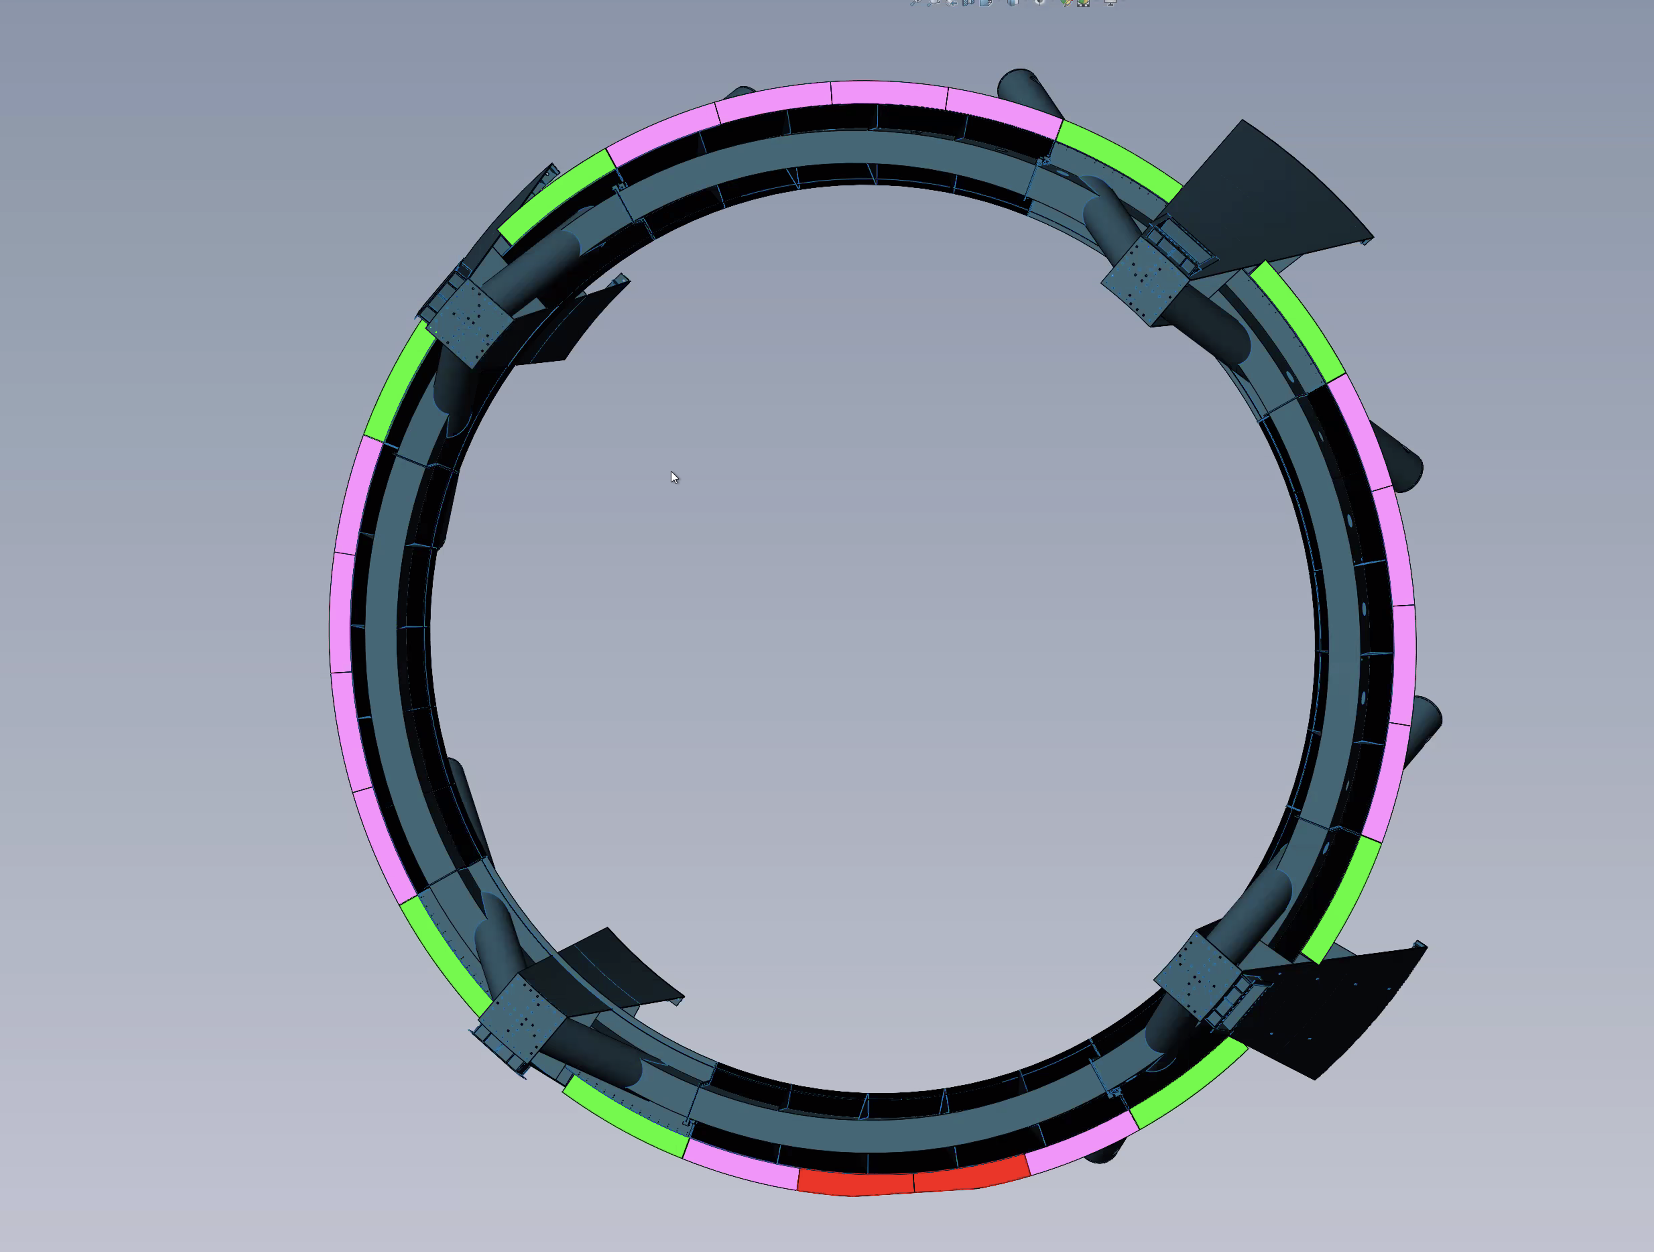
\includegraphics[width=0.7\textwidth, trim={2cm 0cm 0cm 0cm}, clip]{figures/baffle-ring.png}
    \caption{\label{fig:baffle} Initial design of a 220\,mm outward extension to the mid-level light baffle to block the scratched tape light path. The mid-level baffle extension ring is composed of 24 individual panels that can be installed incrementally (colored green, pink, and red in this design drawing).}
\end{figure*}

\section{Conclusions}
\label{sec:conclusions}

The scratched tape stray light feature is caused by illumination from astronomical sources at large (19.8 $\lesssim \theta \lesssim$ 26\,deg) off-axis angles. This light pass through a gap between the mid-level and center-section light baffles on the TMA, bounces off the primary mirror M1, and directly into the camera. These features are prominent visible in LSSTCam images after instrument signature removal and can contribute to down-stream data products such as coadds. Visual inspection has determined that bright instances of the scratched tape feature contribute to at least 5\% of on-sky science images during commissioning and science validation. Instances of these features arising from bright stars can have a surface brightness comparable to $\sim$20\% of the night sky. The LWS is expected to block this light path to the sky once it is installed and commissioned. However, extending the mid-level light baffle outwards by 220\,mm presents a simple and effective stop-gap mitigation strategy in advance of the installation and commissioning of the LWS.

\appendix
% Include all the relevant bib files.
% https://lsst-texmf.lsst.io/lsstdoc.html#bibliographies
\section{References} \label{sec:bib}
\renewcommand{\refname}{} % Suppress default Bibliography section
\bibliography{local,lsst,lsst-dm,refs_ads,refs,books}

% Make sure lsst-texmf/bin/generateAcronyms.py is in your path
\section{Acronyms} \label{sec:acronyms}
\addtocounter{table}{-1}
\begin{longtable}{p{0.145\textwidth}p{0.8\textwidth}}\hline
\textbf{Acronym} & \textbf{Description}  \\\hline

SE & System Engineering \\\hline
\end{longtable}

% If you want glossary uncomment below -- comment out the two lines above
%\printglossaries





\end{document}
